\chapter{Practical Analysis of \textit{sign-to-contract} }
\label{chpr:s2c}
We analysed what are the foundations of \textit{sign-to-contract} from a theoretical prospective, now we want to focus on which are the real reasons that give practical purposes to this technique along with the arising issues.
Finally we show application developed by us that makes possible to create OpenTimestamps proofs with \textit{sign-to-contract}.

\section{Benefits and Issues}
The most relevant feature of \textit{sign-to-contract} is the \textbf{cost} reduction. Each user who is doing a bitcoin transaction can also timestamp with no additional costs, if the transaction is for purpose unrelated to that timestamp the cost is reduced to zero. Such timestamp may be used to prove the existence of an arbitrary high number of files, which does not have to come from the same user.

Since it does not cost anything, someone may decide to include in the signature of one of his transactions the a commitment to the calendar Merkle tip (or, more generally, another aggregation of timestamp requests from a community of clients). 
This is called \textit{external timestamping}.
Then who did the transaction sends to the calendar the information to link the Merkle tip to the transaction.
Now the calendar has all the information to fulfil the timestamp requests from its clients.

If a calendar receives several external timestamp proofs it will increase the timestamping \textbf{frequency}. Clients will have their proof completed in less time and, in some situations\footnote{Miners can always lie about the time they publish on the block, however each user may associate a time to the block header (slightly) different from the one included. For instance, someone running a full node can take note of the time when he first received from the network the block and associate that time to the block header; he is sure that the time he uses is correct for timestamping, since data was created before he received the block, but he will have hard times in convincing others.}, the timestamp can be considered more accurate.

Another benefit of \textit{sign-to-contract} is its \textbf{uncensorability}. 
In fact a \textit{sign-to-contract} transaction is indistinguishable from another one, just like the ones with address commitment; however the latter make the UTXO set bloats, while \textit{sign-to-contract} provides a way to create (almost) uncensorable timestamps without burdening the network.
\begin{table}
\begin{center}
\begin{tabular}{|c| >{\centering}m{2cm} >{\centering}m{2cm} c |}
	\hline
	\textbf{commitment scheme} & \textbf{extra bytes} & \textbf{network friendly} & \textbf{uncensorable} \\ \hline
	address commitment & 33  &  & $\checkmark$  \\ 
	OP\_RETURN & 43  & $\checkmark$ & \\
	\textit{sign-to-contract} & 0 & $\checkmark$ & $\checkmark$ \\ \hline
\end{tabular}
%\captionof{table}{Comparison between commitment schemes, extra bytes are computed considering RIPEMD160 for address commitment and SHA256 for OP\_RETURN.}
\end{center}
\caption[Comparison between timestamping schemes.]{Comparison between timestamping schemes. extra bytes are computed considering RIPEMD160 for address commitment and SHA256 for OP\_RETURN.}
\end{table}

Alongside these benefits there are some issues that should be addressed.
An external actor who is doing external timestamping for a calendar may include some arbitrary data embedded in the proof that he will send back to the calendar, who will include the received part in the complete proofs to distribute to clients. 
However clients expect the calendar to send them clean proofs, if they receive timestamps which have been partially created by external actors they are exposed to new risks, they need to trust that who helped the calendar has not inserted malicious data, for instance virus activators. 
This problem cannot be avoided entirely since \textit{sign-to-contract} proofs always contains arbitrary data by who generates the proof. Such issue could be limited by asking for proof with a strict format, for instance:
\begin{verbatim}
Timestamp: MT
prepend R
secp256k1commitment
prepend TX_p
append TX_a
...
\end{verbatim}
This limits the arbitrariness to only the transaction, in addition it could be limited even more by constraining the number and type of outputs and inputs.

Another issue is the \textit{third party malleability}:
if $(r,s)$ is a valid signature for $(P,m)$ then $(r,n-s)$ is a valid signature too. Once the a \textit{sign-to-contract} transaction is relayed a third party may change it using the above technique, if the new version is mined the timestamp proof must be changed\footnote{This happen with all commitment scheme passing through a non-segwit transaction.}.
%cit segwit source
The malleability problem is solved with \textit{segregated witness} (\textit{segwit}) \cite{BIP141}, however this yield to another issue for \textit{sign-to-contract} proofs.
With segwit two versions of a single transaction are considered. One without the signature (witness) and the other with, the former when hashed produce the TXID the latter the WTXID.
The Merkle root in the block header is a commitment to all the TXIDs, while the WTXIDs are committed in another Merkle tree whose root is inserted in the coinbase transaction. So for a segwit transaction the witness is committed in the block header but the path until there crosses the WTXID Merkle tree, then the coinbase transaction and finally the TXID Merkle tree, as shown in Figure \ref{fig:s2c-segwit}. 
This has two problems: the proof almost double in size (two Merkle tree must be traversed) and the miner may include malicious data in the coinbase. Those are not insuperable issues, still they cause some extra layers of complexity in the implementation.

\begin{figure}
	\begin{center}
		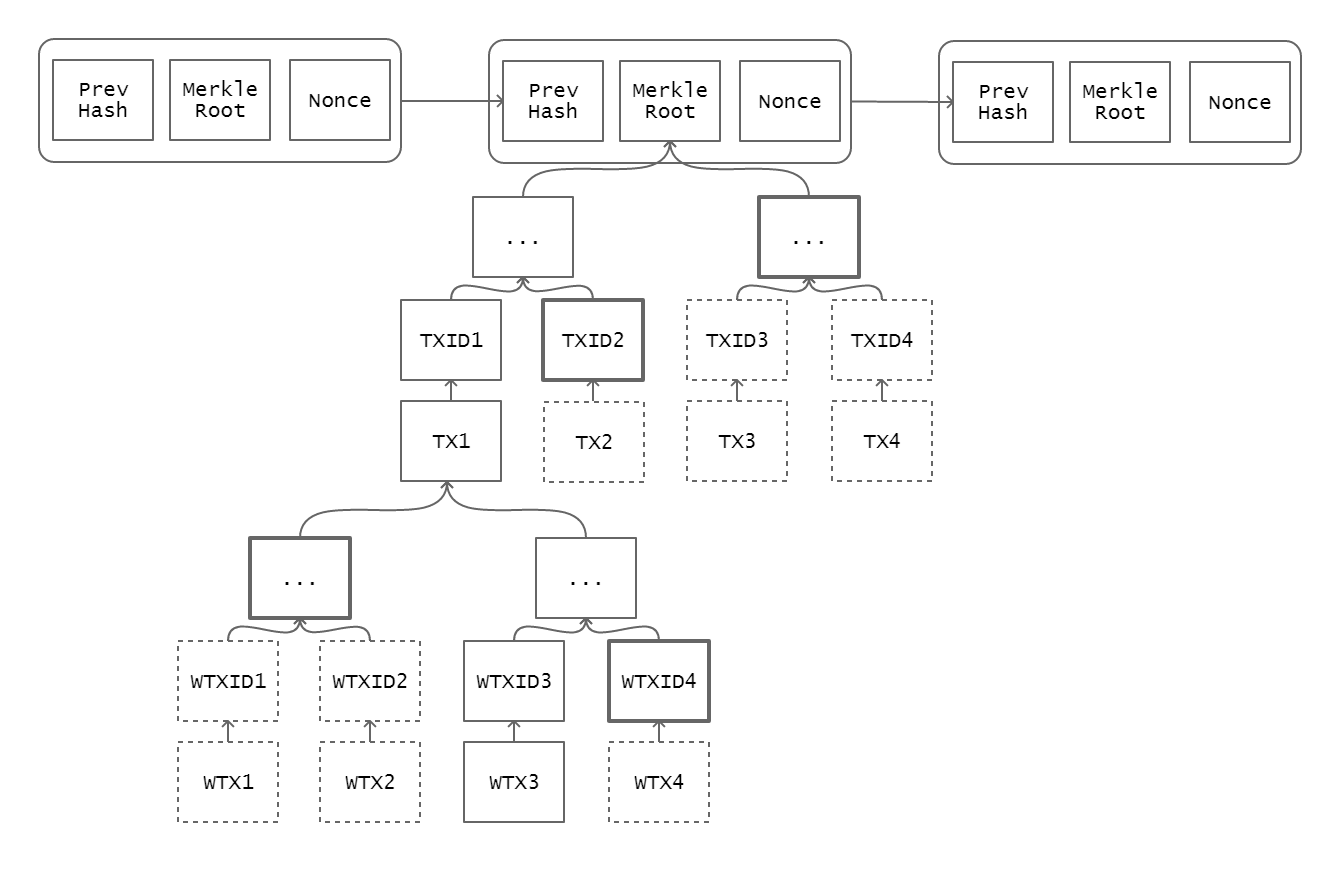
\includegraphics[width=\linewidth]{Images/bitcoin-chain-s2c-segwit.png}
		\caption[\textit{sign-to-contract} with segwit.]{\textit{sign-to-contract} with segwit. The signature is in the transaction with the witness $WTX_3$, which is committed to the coinbase $TX_1$, which is committed to Merkle root.}
		\label{fig:s2c-segwit}
	\end{center}
\end{figure} 


\section{\textit{sign-to-contract} Made Accessible}
The \textit{sign-to-contract} technique can be integrated in every Bitcoin singing software, so that, completely for free, it will also create timestamps.
To make this accessible to everyone we developed a plugin for a popular open source wallet: Electrum \cite{ElectrumWeb} \cite{ElectrumGithub}. 
Electrum is a lightweight wallet, is similar to Simple Payment Verification (SPV) wallets, but instead it asks information to special nodes called the Electrum servers. The wallet, written in python, has very few requirements despite being really flexible, of course it comes at a price: privacy and security are not at the highest standard, unless it is used in very specific ways\footnote{Offline signing and connecting to a personal Electrum server would provide a satisfying but expensive solution.}.
Having said this, it is completely functional for many purposes and it lends itself to host plugins that extend its working, like hardware wallet signing. 
Its features lead our choice to Electrum.

To run Electrum with the plugin it is necessary to use the library python-opentimestamps including \verb|OpSecp256k1Commitment| and to include the plugin among the electrum source files. All the detailed instruction, along with the files constituting the plugin, can be found at \url{https://github.com/LeoComandini/electrum-timestamp-plugin} currently in the experimental branch \textit{s2c}\footnote{The guide to install and run this specific version of the plugin is README-S2C.md and can be found in the experimental branch. For this work refer to commit aef2ee25, in the future we hope to improve the code.}. The reason behind this complicated workaround is that, at this phase, the code is intended for developers for testing purposes, not yet for a general public.

If one is familiar with Electrum code, and if the whole framework of \textit{sing-to-contract} is clear, the implementation is pretty straightforward.  We tried to be the less invasive as possible by using the hooks already present in the code and to keep, this, combined with the deliberate choice to make the code the simplest possible, lead to a suboptimal user experience. 
The signature procedure mimic the standard one adopted by Electrum, the incomplete timestamp and the data necessary to create timestamps is stored in a json file to facilitate debug.
Moreover we do not manage \textit{sign-to-contract} with segwit, since Electrum servers do not support an RPC to retrieve the Merkle path from a transaction with the witness to the coinbase and then to the block header Merkle root.

In Figure \ref{fig:enable-plugin}, \ref{fig:s2c}, \ref{fig:tx-history} and \ref{fig:upgrade} we display few screenshot to give a taste of what the plugin look like.

\begin{figure}
	\begin{center}
		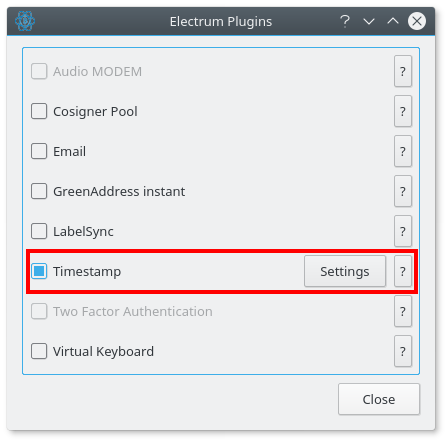
\includegraphics[width=0.5\linewidth]{Images/enable-plugin.png}
		\caption[Enable the plugin to create timestamps.]{Enable the plugin to create timestamps. This will let you select files and create OpenTimestamps proof for them.}
		\label{fig:enable-plugin}
	\end{center}
\end{figure} 

\begin{figure}
	\begin{center}
		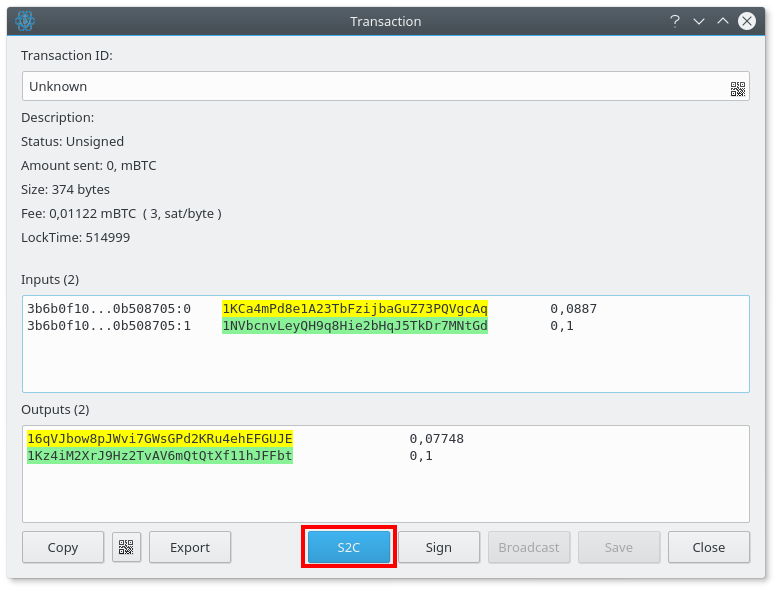
\includegraphics[width=0.9\linewidth]{Images/s2c.png}
		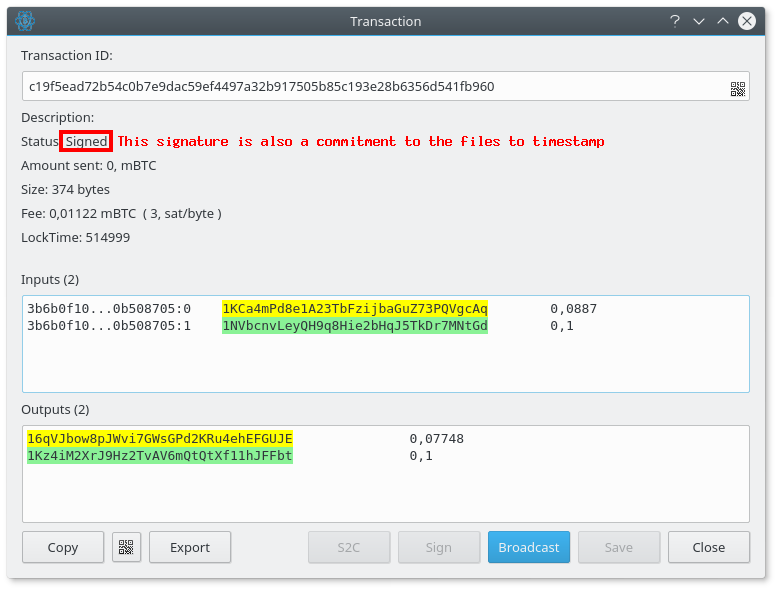
\includegraphics[width=0.9\linewidth]{Images/s2c-done.png}
		\caption[Sign with \textit{sign-to-contract}.]{Sign with \textit{sign-to-contract}. Sign and create a commitment clicking S2C then broadcast the transaction to the network.}
		\label{fig:s2c}
	\end{center}
\end{figure} 

\begin{figure}
	\begin{center}
		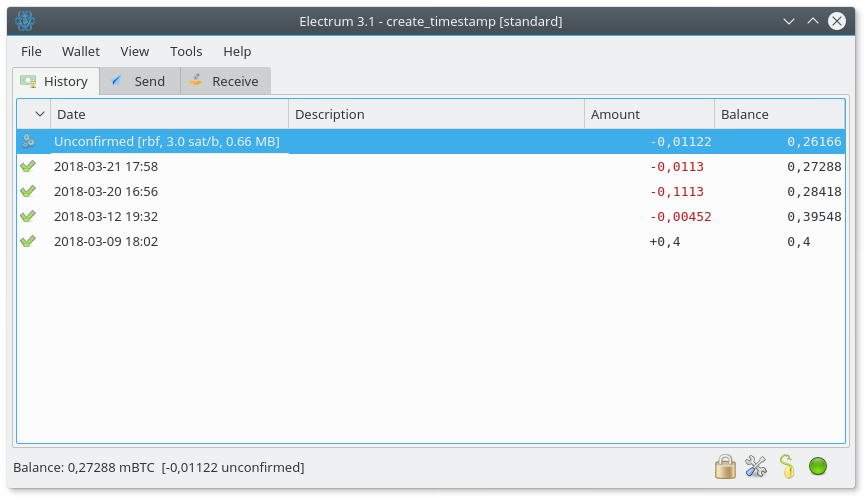
\includegraphics[width=\linewidth]{Images/tx-history.png}
		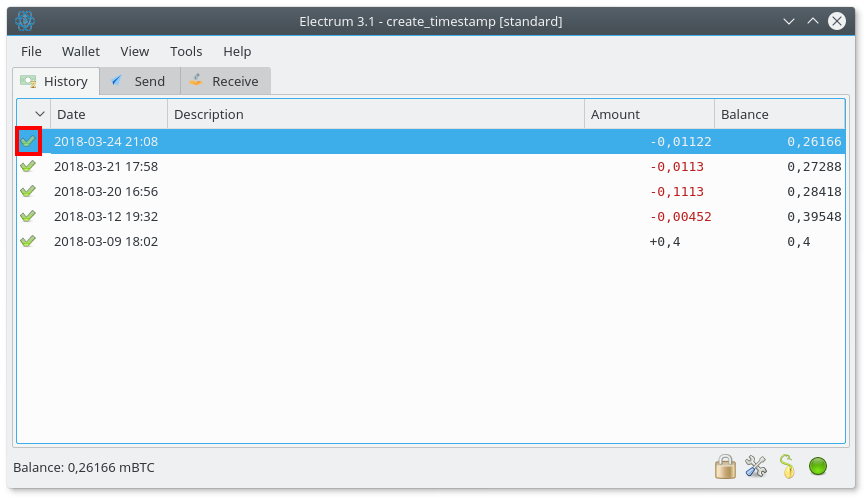
\includegraphics[width=\linewidth]{Images/tx-history-confirmed.png}
		\caption[Transaction history.]{Transaction history. Wait until the transaction is confirmed.}
		\label{fig:tx-history}
	\end{center}
\end{figure} 

\begin{figure}
	\begin{center}
		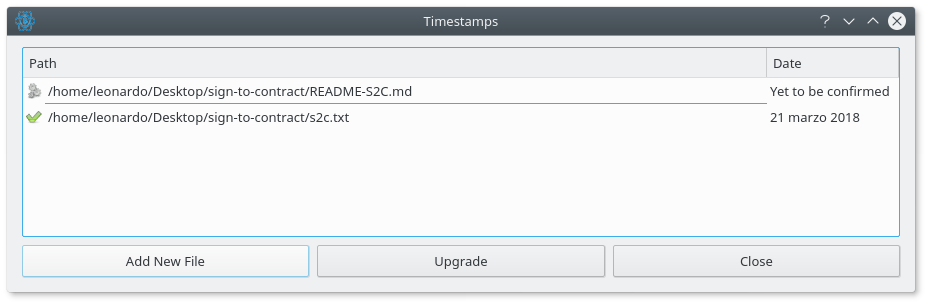
\includegraphics[width=\linewidth]{Images/pending-attestation.png}
		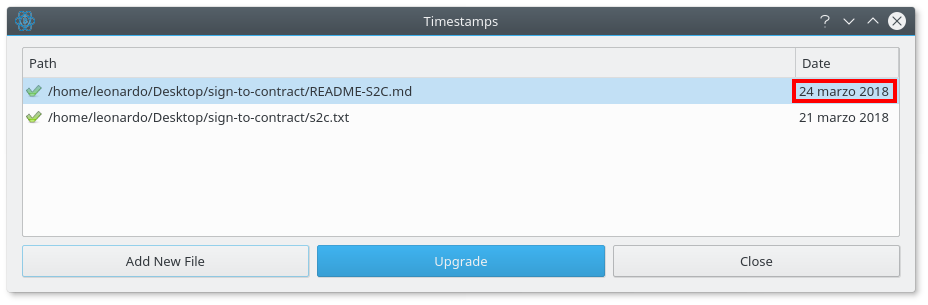
\includegraphics[width=\linewidth]{Images/post-upgrade.png}
		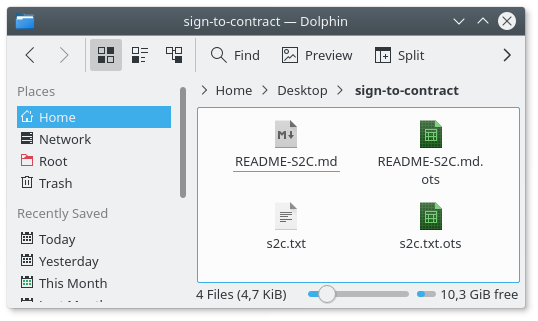
\includegraphics[width=0.7\linewidth]{Images/file-and-ots.png}
		\caption[Complete the timestamp.]{Complete the timestamp. Click on upgrade to terminate the timestamp construction. Then the proof is placed next to the timestamped file.}
		\label{fig:upgrade}
	\end{center}
\end{figure} 


At this stage, where  the \verb|OpSecp256k1Commitment| is not yet part of the standard OpenTimestamps library, the plugin may help testing the timestamping with elliptic curve commitments. 
If and when the improvement proposal will be merged, after in-depth testing has been passed, we may ask to include the plugin in the standard release of Electrum.